\documentclass[a4paper, 12pt]{article}
\renewcommand{\baselinestretch}{1.5}
\usepackage{algorithm}
\usepackage{arevmath}     % For math symbols
\usepackage{algpseudocode}
\usepackage{mathtools}
\usepackage{fontspec}
\usepackage{graphicx}
\usepackage{tabularx}
\usepackage{setspace}
\usepackage{longtable}
\usepackage{amsmath}
\usepackage{unicode-math}
\usepackage{capt-of}
\usepackage{sectsty}
\usepackage{stackengine}
\usepackage{hyperref}
\usepackage{caption}
\usepackage{titlesec}
\usepackage{subcaption}
\usepackage{array,ragged2e}
\usepackage[justification=centering]{caption}
\usepackage[format=hang,font={small,bf},labelfont=bf]{caption}
\usepackage{nomencl}
\usepackage{siunitx}
\usepackage{etoolbox}
\makenomenclature
\usepackage[sorting=none]{biblatex} %Imports biblatex package
\addbibresource{ref.bib} %Import the bibliography file
\defbibheading{References}[\bibname]{%
  \section*{\centering #1}%
  \markboth{#1}{#1}}
\newcommand\xrowht[2][0]{\addstackgap[.5\dimexpr#2\relax]{\vphantom{#1}}}
\usepackage[margin=1in]{geometry}
\usepackage{tocloft}

%  \pagestyle{empty}
\setmainfont{Times New Roman}
\captionsetup[figure]{font={small, bf},labelfont={bf},name={Fig.},labelsep=period}
\renewcommand{\algorithmicrequire}{\textbf{Input:}}
\renewcommand{\algorithmicensure}{\textbf{Output:}}
\renewcommand{\nomname}{\makebox[\linewidth]{Nomenclature}}%
\renewcommand{\contentsname}{\hfill\bfseries\Large Contents\hfill}
\renewcommand{\cftaftertoctitle}{\hfill}
\sectionfont{\fontsize{18}{18}\selectfont}
\setcounter{tocdepth}{4}
\setcounter{secnumdepth}{4}
\titleformat{\paragraph}
{\normalfont\normalsize\bfseries}{\theparagraph}{1em}{}
\titlespacing*{\paragraph}
{0pt}{3.25ex plus 1ex minus .2ex}{1.5ex plus .2ex}

\begin{document}
\pagenumbering{roman}
\setcounter{page}{1}
\tableofcontents
\newpage
\begin{center}
\phantomsection
\listoftables
\addcontentsline{toc}{section}{\listtablename}
\end{center}
\newpage
\begin{center}
\phantomsection
\listoffigures
\addcontentsline{toc}{section}{\listfigurename}
\end{center}
%% This code creates the groups
% -----------------------------------------

\renewcommand\nomgroup[1]{%
  \item[\bfseries
  \ifstrequal{#1}{E}{Non-English Alphabets}{%
  \ifstrequal{#1}{H}{English Alphabets}{%
  \ifstrequal{#1}{I}{Abbreviations}{%
  \ifstrequal{#1}{O}{Other symbols}{}}}}%
]}
% -----------------------------------------
%% This will add the units
%----------------------------------------------
\newcommand{\nomunit}[1]{%
\renewcommand{\nomentryend}{\hspace*{\fill}#1}}
%----------------------------------------------
\newpage
\phantomsection{}
\printnomenclature
\nomenclature[E]{\(\beta\)}{Beta}
\nomenclature[E]{\(\sigma\)}{Sigma}
\nomenclature[E]{\(\sum\)}{Uppercase Sigma}

\nomenclature[H]{\(e\)}{Euler's constant \nomunit{\(2.71828\)}}



\nomenclature[I]{\(ANN\)}{Artificial Neural Network}
\nomenclature[I]{\(ARCH\)}{Autoregressive Conditional Heteroscedasticity}
\nomenclature[I]{\(AUC\)}{Area Under Curve}

\nomenclature[I]{\(BN\)}{Bayesian Network}
\nomenclature[I]{\(CART\)}{Classification and Regression Trees}
\nomenclature[I]{\(DAG\)}{Directed Acyclic Graph}
\nomenclature[I]{\(DT\)}{Decision Tree}
\nomenclature[I]{\(EDA\)}{Exploratory Data Analysis}
\nomenclature[I]{\(GARCH\)}{Generalized Autoregressive Conditional Heteroskedasticity}
\nomenclature[I]{\(KNN\)}{K-Nearest Neighbours}
\nomenclature[I]{\(LCR\)}{Liquidity Coverage Ratio}
\nomenclature[I]{\(LR\)}{Logistic Regression}
\nomenclature[I]{\(LDA\)}{Linear Discriminant Analysis}
\nomenclature[I]{\(MLP\)}{Multilayer Perceptron}
\nomenclature[I]{\(MSE\)}{Mean Squared Error}
\nomenclature[I]{\(NSFR\)}{Net Stable Funding Ratio}
\nomenclature[I]{\(NPA\)}{Non Performing Assets}
\nomenclature[I]{\(RBI\)}{The Reserve Bank of India}
\nomenclature[I]{\(RF\)}{Random Forest}
\nomenclature[I]{\(ROC\)}{Receiver Operating Characteristics}
\nomenclature[I]{\(SVM\)}{Support Vector Machine}
\nomenclature[I]{\(VAR\)}{Value at Risk}
\addcontentsline{toc}{section}{Nomenclature}
\newpage
\begin{center}
\phantomsection
\section*{\centering Abstract}
\addcontentsline{toc}{section}{Abstract}
\end{center}
\textit{
{\fontsize{10pt}{10pt}\selectfont In today's era, the data volume is exploding and each second, new data is created and stored on a server or the cloud. This increases the risk of data breaching. Data breaching is an issue that exists at an enterprise level as well as on a day-to-day basis. Protection of data is of significant importance and biometric verification is a commonly used approach to implement data security. Biometric systems are categorized majorly into two types - unimodal and multimodal systems. Unimodal approaches make use of a single biometric trait including face, fingerprint, gait, voice, etc. However, there exists a high number of limitations to this system thus the multimodal system is adapted. The multimodal system performs the fusion of two or more biometric traits and makes the decision based on it. The fusion approach has various algorithms associated with it. These methods and limitations are analyzed in detail and are followed by references to studies showing their results in the field of biometric systems. <TODO: Replace Abstract>
}
}
\vskip 0.1in
\noindent\
\emph{
{\fontsize{10pt}{10pt}\selectfont \textbf{Keywords:}  Banking - Risk Management - Machine Learning - Credit Score}}

\begin{center}
\newpage
\pagenumbering{arabic}
\setcounter{page}{1}
\section{\centering Introduction}
\end{center}
\vskip 0.25in
The banking industry is an essential part of the global economy handling over 150 trillion U.S Dollars worth of global assets. Amidst the economic recession caused due to the COVID-19 pandemic, the total value of banking-related fraud in India doubled from Rs 71,534 Crores in 2018-19 to Rs 1,38,422 Crores in the fiscal year  2020-21 [1]. Global recessions like the 2008 Financial Crisis and the recent COVID-19 pandemic slows down economic output and put a lot of pressure on financial institutions, especially banks. Having a strong infrastructure to manage and mitigate financial risk becomes crucial to keeping the global economic engine running.
\vskip 0.2in
\noindent
Over the last few decades, advancements in Machine Learning have been extensively utilized to help in risk management tasks. With almost all financial instruments running in a digital form, machine learning models are employed extensively to detect fraud, predict commodity prices, track inflation etc. A lot of research has been done academically and in the industry since the 2008 Financial Crisis to build state of the art models for various risk management activities. This report presents a summary of multiple machine learning techniques that are used to solve a variety of risk management related problems.
\vskip 0.2in
\subsection{Applications}
Risk management is a 17.1 Billion U.S. Dollar industry responsible for handling inflation, financial frauds, cyber threats, market volatility etc. [2]. Machine Learning models significantly improve the accuracy of existing risk management tasks and can do so globally by working on petabytes of data that the banking sector produces daily. Typical applications of machine learning in risk management tasks include:

\begin{itemize}
  \item \textbf{Credit Risk:} Determining if the borrower can repay the loan.
  \item \textbf{Market Risk:} Predicting volatility and movement in commodity and equity markets.
  \item \textbf{Financial Fraud Risk:} Identifying money laundering patterns from transactions.
  \item \textbf{Liquidity Risk:} Identifying stability of sectors before investing in financial instruments
  \item \textbf{Operational Risk:} Detecting Fraud and suspicious transactions
\end{itemize}






\vskip 0.2in
\subsection{Motivation}
Risk Management is essential for a country's economy. The Reserve Bank of India (RBI) reported the presence of about Rs. 900 Thousand Crores of Non-Performing Assets (NPA) in 2020 in the Indian banking sector [3]. These are essentially bank loans that are in default or arrears. This amount of loss is roughly equivalent to the cost to build an international airport in India. Machine Learning plays a monumental role in reducing exposure to such risks, which can significantly impact national and global economies.
\vskip 0.2in
\subsection{Objectives}
This report aims to summarize the work done in risk management in the banking sector from a machine learning point of view. Additionally, this report also presents a case study comparing the performance of different machine learning models to evaluate credit risk on a single dataset.
\vskip 0.2in
\subsection{Organization of Report}
<TODO: Write This>
This report is subdivided into four chapters. The first chapter gives the introduction to biometric authentication, its applications, motivations, and the objective of this report. The second chapter gives a basic understanding of the tasks within the biometric system, a brief explanation of the unimodal and multimodal biometric system followed by terminologies used in biometric authentication. The third chapter contains an in-depth understanding of the various implementations of popular unimodal and multimodal biometric techniques that elevate data security. The final chapter covers the conclusion for the report outlining the machine learning and statistical approaches used for biometric authentication.
\newpage

\section{\centering{Theoretical Background}}
\vskip 0.25in
This chapter is subdivided into two parts. The first part is a brief outline of standard machine learning models and terminologies. The second part explains various terminologies related to finance, banking and risk management.
\vskip 0.2in
\subsection{Machine Learning Algorithms}
\subsubsection{Logistic Regression (LR)}
\begin{center}
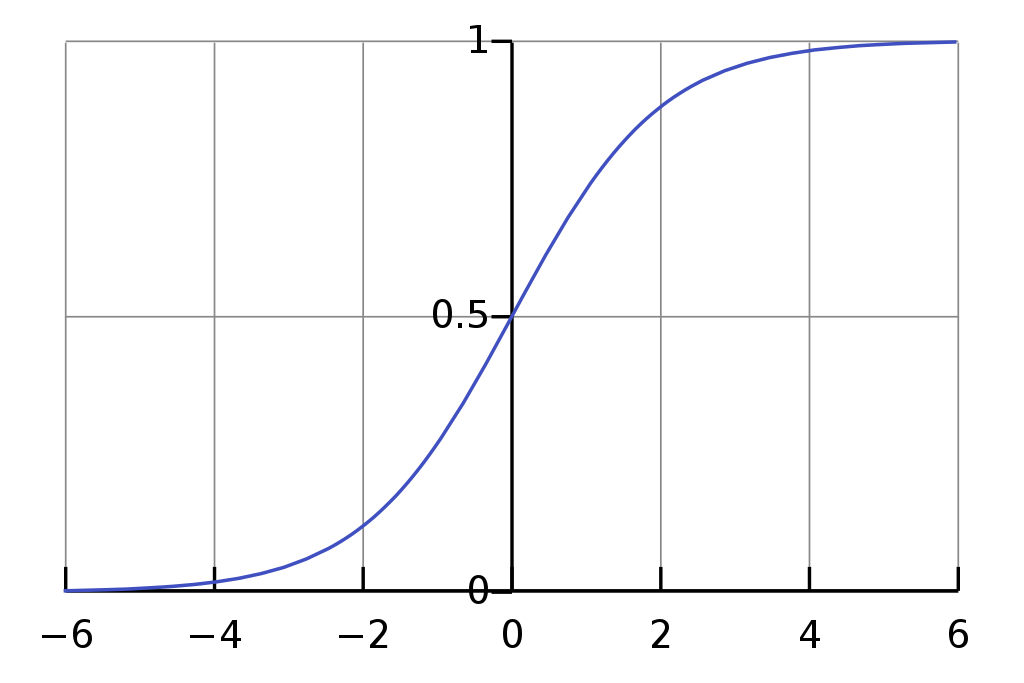
\includegraphics[scale=0.3]{lr.png}
\captionof{figure}{Logistic function curve}
\label{fig:lr}
\end{center}
In statistics, LR models the probability of a specific class or event happening. This probability estimate is further used for binary classification and with minor extensions to perform multi-class classification. The algorithm is based on a logistic function which is a sigmoidal curve. It takes a real-valued input and outputs a number between zero and unity (Fig. \ref{fig:lr}). This output is interpreted as the probability of the task. Mathematically, the logistic function is represented as follows:
\begin{equation}
\sigma(t) = \frac{e^t}{1 + e^t} = \frac{1}{1 + e^{-t}}
\end{equation}
If \(t\) is derived from a single independent linearly varying variable \(x\), the generalized logistic function can be represented as follows:
\begin{equation}
    t = \beta_0 + \beta_1x
    \end{equation}
    \begin{equation}
    p(x) = \sigma(t) = \frac{1}{1 + e^{\beta_0 + \beta_1x}}
\end{equation}
\vskip 0.2in
\subsubsection{Decision Tree (DT)}
\noindent Decision Tree Learning involves the construction of DTs, which will be traversed to conclude a given set of observations of data points. Classification Trees are models where the predicted outcome is discrete. Decision Tree training algorithms work in a top-down fashion to split the data set at every stage using a specific metric. Popular decision trees and their splitting metrics are discussed below.
\vskip 0.2in
\noindent\textbf{Classification and Regression Tree (CART)} \\
\noindent CART model uses the Gini Impurity Index \(I_G\) as its splitting parameter, which is computed for \(j\) classes as follows:
\begin{equation}
    I_{G}(p) = 1 - \sum_{i = 1}^{j} p_i^2
\end{equation}
\vskip 0.2in
\noindent\textbf{Information Gain based DTs} \\
\noindent DT models like ID3, C4.5 and C5.0 use information gain, which is based on the entropy  of the dataset. Mathematically Entropy \(H\) and Information Gain \(IG\) for \(j\) classes are defined as below:

\begin{equation}
    H(T) = - \sum_{i=1}^{j} p_i \log_2 p_i
\end{equation}

\begin{equation}
    IG(T, a) =  H(T) - H(T|a)
\end{equation}

\vskip 0.2in
\subsubsection{Random Forests (RF)}
\noindent RFs are constructed using ensemble learning on DTs. The majority output of the decision trees is considered the output of an RF in a classification task. The mean of all outputs is taken for a regression task. RFs are used as a corrective measure for overfitting of DT based models.

\vskip 0.2in
\subsubsection{Support Vector Machine (SVM)}
\begin{center}
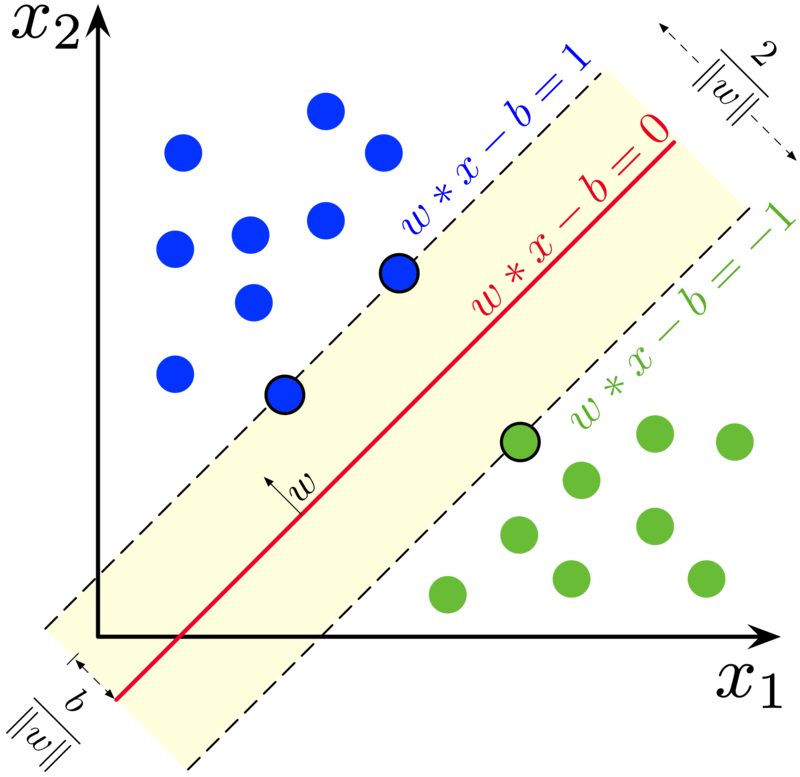
\includegraphics[scale=1.8]{svm-1.png}
\captionof{figure}{Hyperplane construction in SVM}
\label{fig:svm-1}
\end{center}

\noindent SVMs are supervised learning models used for regression and classification tasks. For classification, two hyperplanes are constructed, separating linearly separable data classes. The hyperplane at the midway of these two planes is the maximum hyperplane which acts as a classification boundary (Fig. \ref{fig:svm-1}).

\vskip 0.2in
\begin{center}
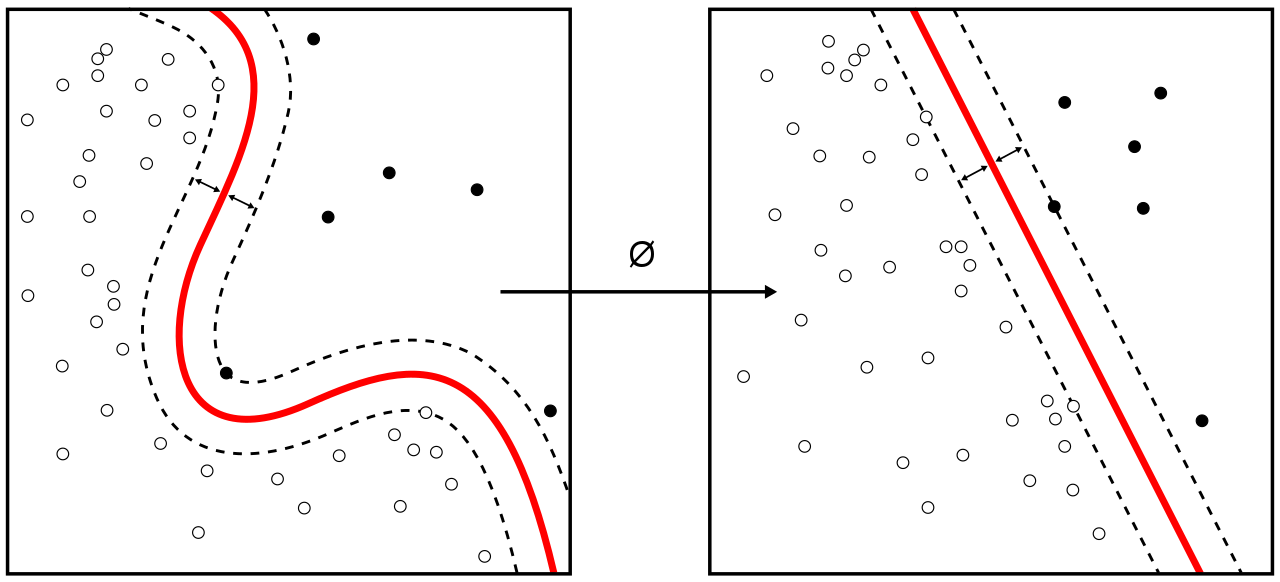
\includegraphics[scale=0.2]{svm-2.png}
\captionof{figure}{Kernel mapping to linear boundaries}
\label{fig:svm-2}
\end{center}
\noindent 
For non-linear data, a kernel is used, which is a function mapping the data into higher dimensional linear feature space (Fig. \ref{fig:svm-2})


\vskip 0.2in
\subsubsection{K-Nearest Neighbours (KNN)}
\begin{center}
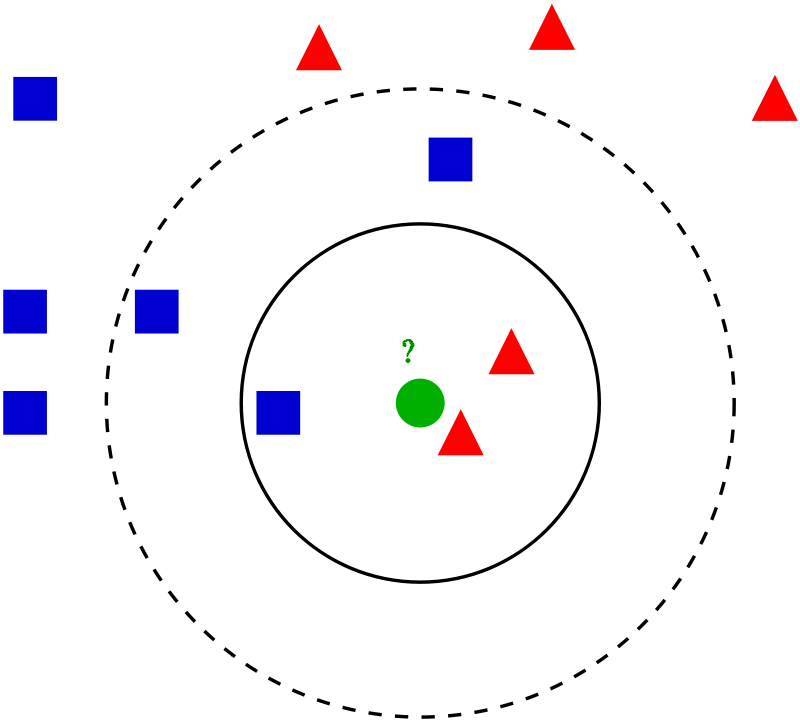
\includegraphics[scale=0.3]{knn.png}
\captionof{figure}{Example of KNN}
\label{fig:knn}
\end{center}
\noindent KNN is a supervised algorithm for supervised classification and regression tasks. KNN works by finding the \(K\) closest data points to a given query point. The output is the most frequent label for classification and the mean of the label for regression tasks. The value of \(K\) is user-defined as a hyperparameter, and the distance metric is euclidean or hamming distance depending on the context of the dataset.

\vskip 0.2in
\subsubsection{Bayesian Network (BN)}
\noindent A BN is a Directed Acyclic Graph (DAG) used to represent the probabilistic dependencies of a collection of random variables. Each node of the BN represents a random variable, and each edge between the nodes represents the conditional probability between the nodes, which is derived from the Bayes theorem:
\begin{equation}
    P(A|B) = \frac{P(B|A)P(A)}{P(B)}
\end{equation}
As an example, consider the BN in (Fig. \ref{fig:bn}), modelling the conditions when the grass can be wet. If it rains or the sprinklers are active, there is a higher probability of grass being wet. Moreover, if it is raining, the probability of the sprinkler being kept active is lesser.
\begin{center}
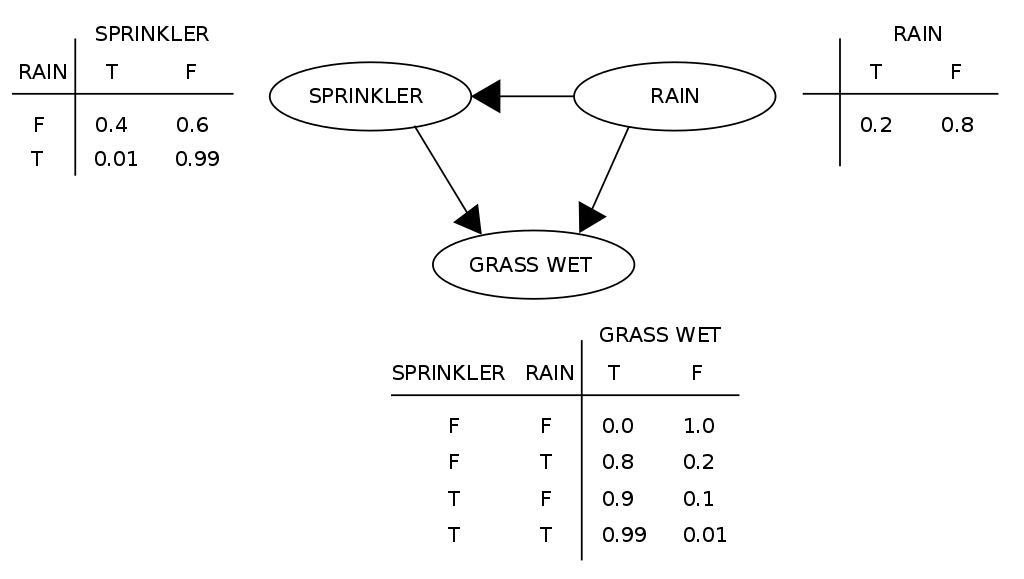
\includegraphics[scale=0.3]{bn.png}
\captionof{figure}{Example of BN}
\label{fig:bn}
\end{center}

\vskip 0.2in
\subsubsection{Linear Discriminant Analysis (LDA)}
\begin{center}
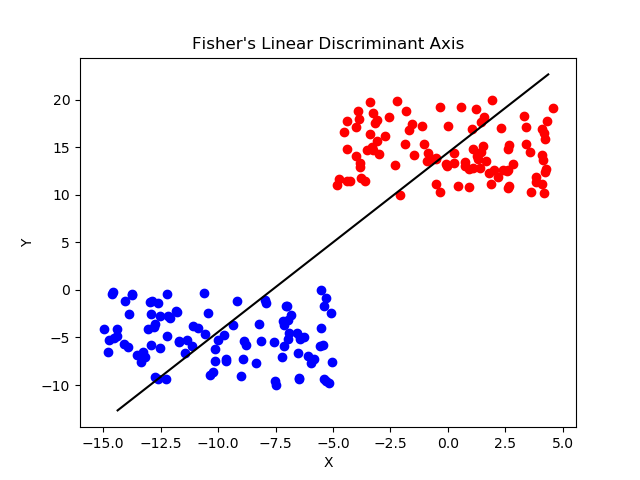
\includegraphics[scale=0.8]{lda.png}
\captionof{figure}{Fisher's LDA Visualization}
\label{fig:lda}
\end{center}

\noindent LDA is used for dimensionality reduction, especially for supervised classification tasks to separate two or more classes spatially. LDA takes a component of the data points on a single axis tuned to maximize the distance between two classes and minimize the variation within members of a single class.

\vskip 0.2in
\subsubsection{Artificial Neural Networks (ANN)}

\noindent ANNs are machine learning models mimicking biological neural networks. An ANN consists of neuron layers where each layer contains an array of artificial neurons. These neurons are essentially mathematical functions that take input values from previous layers and are tunable using a set of weights and biases. ANNs are used for supervised, unsupervised as well as reinforcement learning tasks.

\begin{center}
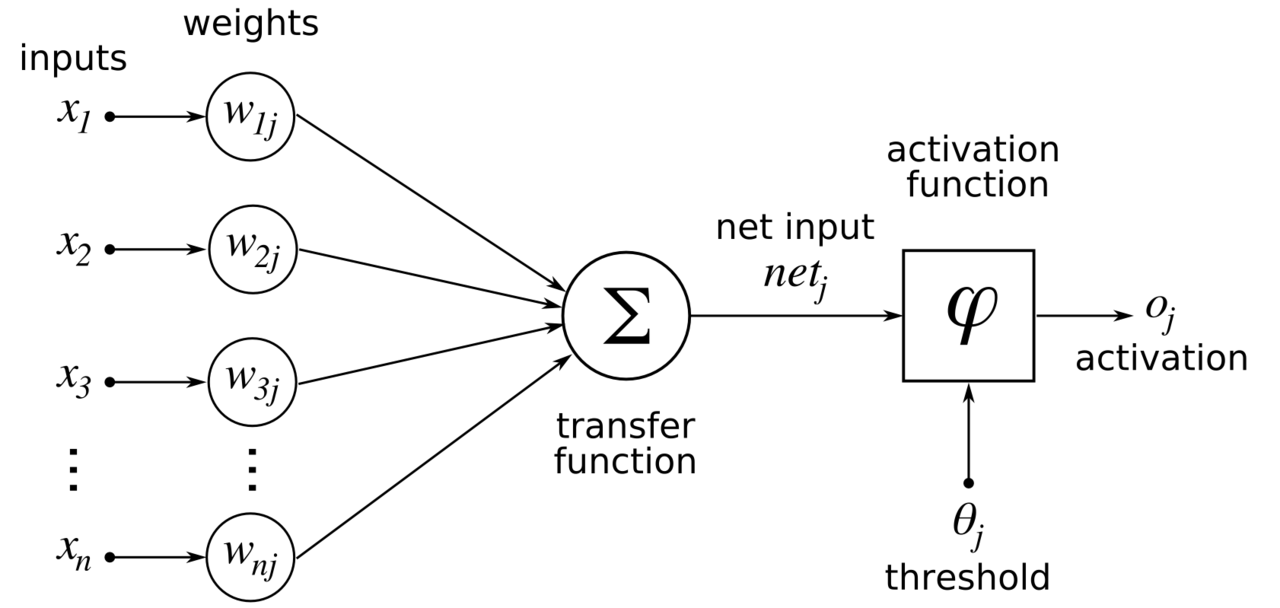
\includegraphics[scale=0.38]{ann.png}
\captionof{figure}{Single neuron in an ANN}
\label{fig:ann}
\end{center}

\vskip 0.2in
\noindent\textbf{Multilayer Perceptron (MLP)} \\
\noindent MLPs are a class of feedforward ANNs where the connections between layers of neurons are unidirectional and acyclic. Each neuron is an activation function like hyperbolic tan, logistic function and rectifier function.
\begin{equation}
    y(v_i) = \tanh(v_i)
\end{equation}
\begin{equation}
    y(v_i) = \frac{1}{1 + e^{v_i}}
\end{equation}
\begin{equation}
    y(v_i) = \max(0, v_i)
\end{equation}

\vskip 0.2in
\subsection{Overview Banking and Risk Management Terminologies}
\subsubsection{Risk}
\noindent Risk in finance is defined as uncertainty or volatility of unexpected outcomes, representing the value of assets, equity, or earnings. This includes both positive as well as negative outcomes. A higher return is associated with a more significant variability of outcomes [6]. Risk is broadly classified into Credit Risk, Market Risk, Liquidity Risk and Operational Risk.

\vskip 0.2in
\subsubsection{Market Risk}
\noindent Market risk is the risk of the movement of market prices. Prices of market parameters that fluctuate randomly include equity indexes, commodity prices, interest rates and foreign exchange rates [4].

\vskip 0.2in
\noindent\textbf{Time Series Forecasting} \\
\noindent Time Series Forecasting is used to predict the market price movement. It involves conceptualizing statistical and machine learning models to predict future values based on previously observed values.

\vskip 0.2in
\noindent\textbf{Innovation} \\
\noindent Innovation is the difference between a forecast made by a statistical algorithm and the actual value for a time-varying function.

\vskip 0.2in
\noindent\textbf{Heteroscedasticity} \\
\noindent Heteroscedasticity is the variance or volatility observed in a time-varying random function.

\vskip 0.2in
\subsubsection{Liquidity Risk}
\noindent Liquidity is the ease with which a financial instrument can be exchanged for money without losing value. High liquidity indicates a high supply and demand for an asset, which means there will always be buyers and sellers. Liquidity risk is the uncertainty linked with the outcome and possible losses of such an asset transaction into funds [7].

\vskip 0.2in
\noindent\textbf{Measuring Liquidity} \\
\noindent Liquidity is measured using ratios like Liquidity Coverage Ratio (LCR) and Net Stable Funding Ratio (NSFR). LCR measures the number of liquid assets a bank has to cover for any short term liquid fund requirements. NSFR, on the other hand, measure a bank's long term resilience to liquidity risks. Basel Norms require that both the ratios must be maintained above 100\% by banks.

\begin{equation}
    LCR = \frac{\text{stock of high quality liquid assets}}{\text{total net cash} - \text{flow over the next 30 days}}
\end{equation}

\begin{equation}
    NSFR = \frac{\text{available amount of stable funding}}{\text{required amount of stable funding}}
\end{equation}

\vskip 0.2in
\subsubsection{Operational Risk}
\noindent Operational Risk is the risk associated with failures in internal procedures, external events, and infrastructure. Fraud detection, cyber security attacks, suspicious transaction detection, money laundering all come under the radar of operational risk [4].

\vskip 0.2in
\noindent\textbf{Money Laundering} \\
\noindent Money Laundering converts substantial amounts of funds earned from crimes and terrorism into origination from a legitimate source. This is accomplished by routing transactions through numerous layers of legal transactions to hide the natural source of income.

\vskip 0.2in
\subsection{Summary}
In conclusion, this chapter briefly introduces various concepts and terminologies that would be a prerequisite for Chapter 3 and Chapter 4. Machine learning algorithms are used to solve a vast array of economics, banking, and risk management problems.

\newpage
\section{\centering Literature Review}
\vskip 0.25in
This chapter attempts to provide an in-depth understanding of the different machine learning approaches that have been used for the verification and recognition process of biometric traits. The following chapter is divided into 2 subsections - unimodal system and multimodal system. Within these subsections, a brief understanding is provided of the approaches used for biometric recognition and verification.
\vskip 0.2in
\subsection{Unimodal Biometric Verification System}
This subsection provides an in-depth understanding of the various unimodal biometric traits and the approaches used for the verification of these biometric traits.
\vskip 0.2in
\subsubsection{Common Biometric Traits}
Biometrics traits including face, voice, fingerprint, etc are few of the most commonly-used biometric traits.
\vskip 0.2in
\paragraph{Deoxyribonucleic acid (DNA)}
DNA is a unique code for each individual and is a one-dimensional vector in shape. The one catch is that identical twins have indistinguishable DNA patterns; nevertheless, with 26 distinct bands analysed, the likelihood of two individuals having the same DNA profile is less than one in a hundred billion \cite{bashir:2015}. The DNA detection/verification is carried out through polymorphism analysis. The following figure (Fig. 10) explains the basic flow to DNA polymorphism analysis.
\begin{center}
\includegraphics[scale=0.8]{dna authentication.jpeg}
\captionof{figure}{The flow of DNA polymorphism analysis \cite{masaki:2011}}
\end{center}
\vskip 0.2in
\noindent The limitations associated with this trait include \cite{jain:2004}: 
\begin{enumerate}
\item \textbf{Contamination and Sensitivity} \vskip 0.05in \noindent It's simple to steal a strand of DNA from a certified identity and use it for nefarious purposes.
\item \textbf{Automatic real-time recognition issues} \vskip 0.05in \noindent The present DNA matching methods involve various chemical processes. This requires the use of an expert's skills and is not a real-time process.
\end{enumerate}
\vskip 0.2in
\paragraph{Face}
Individuals are recognized based on the structure of their faces. Each face is made up of peaks and valleys and has features located at varying latitudes and longitudes of the face as seen in figure (Fig. 11). Within this, a face scanner acts as the sensor and it is used for the enrollment of an individual face trait and can be further used for verification \cite{oloyede:2016}. 
\vskip 0.2in
\begin{center}
\includegraphics[scale=0.6]{face marks.png}
\captionof{figure}{Human face with peaks and valleys at different altitude \cite{oloyede:2016}}
\end{center}
\vskip 0.2in
\noindent The face recognition/verification process has advanced from the simple geometrical matching of the latitude and longitude to complex mathematical representations, providing higher accurate results. There have been several research works and approaches in the field of face verification systems. Broadly, the use of the neural network, SVM classifiers, PCA for dimensionality reduction, and various deep network implementations has been carried out in the field.  
\vskip 0.2in
\noindent A face detection system based on a neural network and the color of skin has been implemented. This system showed successful detection of faces on videos and photos. Another implementation used SVM for detecting a face. Here, an elastic graph matching was used for locating feature points of facial images. This system showed effectiveness for the face recognition system \cite{oloyede:2016}. Different lighting and poses for the face can pose a major problem in face recognition. It was solved by employing a deep convolutional neural network (CNN) to optimise the embedding rather than an intermediate bottleneck layer as in earlier DL approaches. \cite{schroff:2015}. However, using face recognition as an individual trait has various limitations that remain unsolved. 
\vskip 0.2in
\paragraph{Fingerprint}
Fingerprints are one of the most commonly adapted biometric authentication techniques. They have unique features associated with them and are unique for identical twins as well. Fingerprints constitute ridges and valleys as seen in figure (Fig. 12). The ridges make up the minutiae points upon which the recognition/verification of fingerprints is performed \cite{bashir:2015}.
\vskip 0.2in
\noindent Few approaches that have shown significant accuracy for fingerprint verification have been stated. A fingerprint matching approach has been proposed based on the Hidden Markov Model (HMM) approach. Another approach for embedding a double watermark into fingerprint images was proposed. This approach enhanced the authentication performance based on watermark messages \cite{oloyede:2016}.
\vskip 0.2in
\begin{center}
\includegraphics[scale=0.6]{fingerprint.png}
\captionof{figure}{Ridges and valleys of a fingerprint \cite{oloyede:2016}}
\end{center}
\vskip 0.2in
\noindent This trait's drawbacks include the following \cite{jain:2004}: 
\begin{enumerate}
    \item Fingerprint can introduce noisy data as dirt on a fingerprint can change the feature provided by the trait.
    \item Spoofing attacks can easily cause one to steal the fingerprint identification of the individual and use it for wrong intent.
    \item It requires a large number of computational resources, especially for the identification mode.
\end{enumerate}
\vskip 0.2in
\paragraph{Voice}
The voice is a biometric traits that combines behavioral and physiological characteristics. The shape and size of an individual's vocal tracts, nasal activities, etc are used to extract details from their voice. \cite{jain:2004}. 
\vskip 0.2in
\noindent A system known to verify a customer in a short time was developed by Barclays using speaker recognition. To extract features, the detection of nodules was implemented using a larynx pathology classifier. The classifier was based on linear prediction coefficients, least squares support vector machines \cite{oloyede:2016}. This method provided an overall accuracy of 90\% The limitation associated with this trait is it has a high FRR \cite{bashir:2015}. 
\vskip 0.2in
\subsubsection{Unique Biometric Traits}
Unique biometric traits include utilizing brain waves and heartbeats for biometric authentication as novel approaches.
\paragraph{Brain}
The analysis of the firing of neurons within the brain and various brain activities can serve as a novel approach to biometric authentication. The use of electroencephalogram (EEG) is a unique approach.Researchers have proposed employing autoregressive models (AR) to model the EEG signal. For classification, Kohonen's Vector Quantizer (VQ) and discriminant analysis have been proposed. Recently, the use of Gaussian Mixture Models (GMM) has proved to serve as an alternative to classification \cite{bashir:2015}.
\paragraph{Heart}
Heartbeats follow the characteristics of a biometric system such as distinctiveness, universality, etc. An electrocardiogram (ECG) evaluates and tests the heartbeats and using it as an authentication mode has the advantage of adopting live user body signals. In general, machine learning algorithms are adopted for constructing the verification model by getting the individual's live ECG data. However, several challenges exist for constructing the model from ECG signal such as pre-processing for data quality, selecting the best machine learning approaches.
\vskip 0.2in
\noindent Kim et al. propose an algorithm in which the ECG signal is pre-processed using baseline drifting adjustment and other methods followed by subjecting it to the ML algorithms \cite{kim:2019}. The ML algorithms are subdivided into regression-based in which SVM and DT are tested and classification based in which ANN and CNN are tested. It has been discovered that DT performs best for ECG-based user authentication. The following figure (Fig. 13) shows the algorithm proposed for individual verification using ECG data. 
\vskip 0.2in
\begin{center}
\includegraphics[scale=0.95]{heart algo.png}
\captionof{figure}{Algorithm for ECG biometric authentication \cite{kim:2019}}
\end{center}
\subsubsection{Summary}
The following table (Table 1) shows the accuracy of various common unimodal biometric traits against the various characteristics of a biometric system such as Continuity, Performance, etc.
\vskip 0.2in
\begin{table}[h!]
\caption{Comparison of various biometric techniques.  
High, Medium, Low are denoted by H, M and L \cite{jain:2004}}
\label{table:1}
\vskip 0.05in
\begin{tabularx}{1.0\textwidth} { 
  | >{\raggedright\arraybackslash}X 
  | >{\raggedright\arraybackslash}X 
  | >{\raggedright\arraybackslash}X
  | >{\raggedright\arraybackslash}X
  | >{\raggedright\arraybackslash}X|}
 \hline
 \textbf{Biometric Identifier} & \textbf{Universality} & \textbf{Distinctiveness} & \textbf{Performance} & \textbf{Collectability} \\
 \hline
 DNA & H & H & H & L \\
 \hline
 Face & H & L & M & H \\
 \hline
 Fingerprint & M & H & H & M \\ 
 \hline
 Voice & M & L & L & M \\
 \hline
\end{tabularx}
\end{table}
\vskip 0.1in
\noindent The table shows that a unimodal biometric trait doesn’t provide highly desirable results and hence, the multimodal system was adapted which uses the individual which will be further elaborated in the report.
\vskip 0.2in
\subsection{Multimodal Biometric Verification System}
The most prevalent method for fusing multimodal data is fusion at the score level. The fusion scoring techniques are subdivided into two approaches - combination and classification \cite{telgad:2014}. The fused score for the combinational technique is derived by normalizing the incoming matching score of the various biometric data. For the classification approach, fusion classifiers are used where the input to this classifier is the matching scores of the various biometric data. These classifiers then help with the decision of whether the identity is verified or an imposter.
\vskip 0.2in
\subsubsection{Score-level fusion: Combinational Approach}
Telgad et al. have come with a combination approach for fusion at score level in a multimodal biometric system. The approach makes use of the combination of face and fingerprint biometric traits \cite{telgad:2014}. The subsection explains the separate methods used for score extraction and the combinational method proposed.
\noindent\paragraph{Face recognition (PCA)} 
\noindent The paper puts forward the use of PCA for the feature extraction of face modalities. PCA only extracts the relevant information from the face and this algorithm is majorly used for dimension reduction. 
\vskip 0.2in
\noindent By treating the image in high dimensional space, the algorithm makes use of eigenvectors and covariance matrix to get the feature vector representing the image. To get the matching score for the feature vector, Euclidean distance is applied to the database. This score is then normalized to be used further for the combinational approach. The accuracy obtained for this method is 92.8\%.
\noindent\paragraph{Fingerprint recognition (Minutiae matching)} 
\noindent As discussed in the above section (Sec 3.1.3), fingerprints constitute ridges and valleys. These, upon scanning, are converted to ones and zeros.  Furthermore, complex algorithms work on identifying the characteristics of fingerprints, known as minutiae. The minutiae are stored within the template in the database. For identification or verification purposes, a subset of it needs to be matched with the incoming query image.
\vskip 0.2in
\noindent In the verification process, the fingerprint is scanned for the individual and is preprocessed and the minutiae points are detected for the same. Once detected, the matching is done with the euclidean distance matcher and the similarity score is extracted. Let A = \{$m_1$, $m_2$, ..., $m_n$\} and B = \{$m_1$, $m_2$, ..., $m_n$\} be a set of minutiae points extracted from the database and the query images, where $m_i$ = $\{x, y, θ\}$ where x and y are the cartesian coordinates of the minutiae points and θ is the orientation between the points.
\vskip 0.1in
\begin{align}
sd = \sqrt{((x_j - x_i)^2) + ((y_j - y_i)^2)} \le r_o
\end{align}
\begin{align}
dd = min(\mid (\theta_j - \theta_i) \mid, 360 - \mid (\theta_j - \theta_i) \mid) \le \theta_o
\end{align}
\vskip 0.1in
\noindent Minutiae in A and B are said to be matched if the spatial distance (Eq. 3) between them is smaller than a given tolerance and the direction difference  (Eq. 4)  between them is smaller than the angular tolerance. The pairing then generates a similarity score based on the matching and is normalized for the purpose of fusion. The accuracy achieved with this method is 93\%.
\noindent\paragraph{Fingerprint recognition (Gabor Filter approach)} 
\noindent The filter-based formula uses a bank of Gabor filters to capture the native and global details of a fingerprint. The matching is then performed through a euclidean distance intermediator between the finger codes of the query image and the database. This approach gave an accuracy of 95\%.
\noindent\paragraph{Combinational Approach} 
\noindent Let $MS_{face}$, $MS_{finger1}$, and $MS_{finger2}$ be the matching scores obtained from face and fingerprint modalities respectively. The steps involved for the fusion at score level are: 
\begin{enumerate}
    \item \textbf{Score Normalization} \vskip 0.05in \noindent Min-max normalization method is used to scale/normalize each score between the range of 0 and 1 where the min and max value correspond to the minimum and maximum matching score for the particular trait. The normalization score of the traits are denoted as $N_{face}$, $N_{finger1}$, $N_{finger2}$. The equations (Eq. 5-7) shows how the normalized scores are calculated. \begin{align}
        N_{face} = \frac{MS_{face} - min_{face}}{max_{face} - min_{face}}
    \end{align}
    \begin{align}
        N_{finger1} = \frac{MS_{finger1} - min_{finger1}}{max_{finger1} - min_{finger1}}
    \end{align}
    \begin{align}
        N_{finger2} = \frac{MS_{finger2} - min_{finger2}}{max_{finger2} - min_{finger2}}
    \end{align}
    \item \textbf{Generation of Similarity Scores} \vskip 0.05in \noindent The normalized score obtained for the face is through PCA while that for the fingerprint is a similarity score. For the fusion of scores, each score needs to be either a similarity or dissimilarity measure.
    \item \textbf{Fusion of Score}
    \begin{align}
        MS = \alpha * N_{face} + \beta * N_{finger1} + \beta\textit{1} * N_{finger2}
    \end{align} \noindent From the above equation (Eq. 8), α, β, and β1 are three weight values associated with the normalized scores of the face and the fingerprints. A combination of linear or exponential functions has been used. The value of the matching score (MS) is used as the matching score. If the MS value is above a threshold, the identity is considered to be legitimate else an imposter.
\end{enumerate}
\noindent\paragraph{Result} 
\noindent Within this paper, the fusion at a scoring level using the combinational approach shows a significant improvement in the verification process of an identity than the statistical rule-based methods. In the combinational approach, the accuracy reaches 97\% which is higher than all the individual biometric trait accuracy scores.
\vskip 0.2in
\subsubsection{Score-level fusion: Classifier Approach}
Damousis et al. has written a comparative study of various classification algorithms that are used for the fusion at score level. The study uses the combination of the face and speech biometric traits. The sub-section explains the classifiers used in the study and their respective FAR and FRR followed by a conclusive result \cite{damousis:2012}.
\noindent\paragraph{SVM} 
\noindent In this, the SVM classifier combines the matching scores of multi-dimensional vectors of various biometric data. The radial basis kernel function (RBF) has been utilized in this study. The RBF is chosen to handle the non-linear data and it requires lesser hyperparameter tuning. Through experimentation on hyperparameter values, the final trained model was tested. After testing, the SVM model achieved the best performance on the test data with 0\% FAR and 0.25\% FRR.
\noindent\paragraph{Gaussian Mixture Model (GMM)} 
\noindent Bayesian classification is based on probability theory and chooses an output based on the most probable or least risk option. A Gaussian distribution provides a good approximation for class model shape in a given feature space. Gaussian distribution works on the assumption that the class model is a model of one class only but if the system is multimodal, the Gaussian distribution cannot capture the underlying information. Thus, in this study, the GMM model is introduced \cite{damousis:2012}. This model is a mixture of several Gaussian distributions and can represent different subclasses within a class. On creation and testing of the model, the GMM model achieved performance on the test data of 0.028\% FAR and 1\% FRR.
\noindent\paragraph{Artificial Neural Network (ANN)} 
\noindent The NN is a three-layer forward network in which there are N input neurons, Y hidden neurons, and a single output neuron. The N is equal to the number of the unimodal biometric data that is being used for fusion and Y is set through experimentation. After applying bias on each neuron and setting all the hyperparameters, the model is trained. The final model is tested and after testing, the NN model achieved a performance on the test data with 0\% FAR and 1\% FRR.
\noindent\paragraph{Result} 
\noindent Within this study, the fusion at a scoring level using the classification approach shows a significant improvement in the verification process of an identity than the statistical rule-based methods and the unimodal methods.
\vskip 0.2in
\subsection{Summary}
The literature review is subdivided into unimodal and multimodal biometric systems. Under the unimodal biometric system, it covers an in-depth explanation of the existential machine learning approaches for the verification of the biometric traits (DNA, fingerprint, face, and voice) and their limitations. The multimodal biometric system covers an in-depth about the approaches for the fusion at the score level. 
\newpage
\section{\centering Conclusion}
\vskip 0.25in
In today's era, the data volume is exploding and each second, new data is created and stored on a server or the cloud. This increases the risk of data breaching and the need for data security. The report outlines the method and approaches by which biometric authentication helps with the verification of identity. This further helps in preventing data breaching by allowing authorized personnel for specific data usage. Furthermore, the report outlines the advancements in biometric authentication from unimodal systems to multimodal systems. The evaluation characteristics of the biometrics system include universality, performance, etc, and evaluation metrics such as EER, FAR, and FRR is outlined in the report. Based on these evaluations, the performance of the system was understood and it is observable that the multimodal systems perform better than the unimodal system. 
\vskip 0.2in
\noindent Among the unimodal systems, various approaches and research has been discussed for face, fingerprint, DNA, brain, heart, and voice verification. It is observable that fingerprint is one of the most common approaches and both face and fingerprint have had advancements in their verification approach. It makes use of deep learning models, SVM classifiers and convolutional models, etc. Among the various classifiers and regression models, it is observed that SVM classifiers perform the best for verification purposes except for heart biometric verification where DT supersedes SVM in performance.
\vskip 0.2in
\noindent Among the multimodal systems, the approaches under fusion at the scoring level have been discussed. For each approach, i.e., classification and combination, research has been discussed and outlined in the report. For the combinational approach, the process is neatly outlined on how the matching score is calculated based on the normalization score of each biometric trait. For the classification approach, various classifiers have been tested such as SVM, GMM, and ANN where SVM supersedes the other fusion classifiers in performance in terms of FAR and FRR.  With the current pace of advancement in technology, significant improvements within the field of unimodal and multimodal biometric systems are expected. 

\newpage
% \textbf{
% {\fontsize{18pt}{18pt}\selectfont References} 
% }\\
% \addcontentsline{toc}{chapter}{References}
% \printbibliography
\phantomsection
\addcontentsline{toc}{section}{References}
\printbibliography[heading={References}, title=References]
\newpage
\phantomsection
\section*{\centering Acknowledgment}
\addcontentsline{toc}{section}{Acknowledgment}
\vskip 0.2in
\raggedright I would like to express my deep gratitude and indebtedness to my seminar guide, Dr. Sankita J. Patel, Assistant Professor, Computer Engineering Department, SVNIT Surat for her valuable guidance, useful feedback and co-operation with a kind and encouraging attitude for the successful completion of this report. I would also like to express a deep sense of gratitude to the Computer Engineering Department faculties for direct or indirect support for the completion of this seminar.
\end{document}
